\subsection*{Kategorisering af KOL-patienter} \label{sec:kategorisering}
KOL-patienter skal have en individuel kategorisering, dette er nødvendigt for således at sikre patienter får en træning tilpasset til deres niveau. Kategoriseringen forekommer ved registrering og kan efterfølgende redigeres.
Hertil inddeles patienter i ABCD-kategorisering, der er beskrevet i \autoref{sec:klassifikation}. Af \autoref{fig:Kate} ses aktivitetsdiagrammet for kategoriseringen.

\begin{figure} [H]
\centering
\textbf{Aktivitetsdiagram: Kategorisering af KOL-patienter}\par\medskip
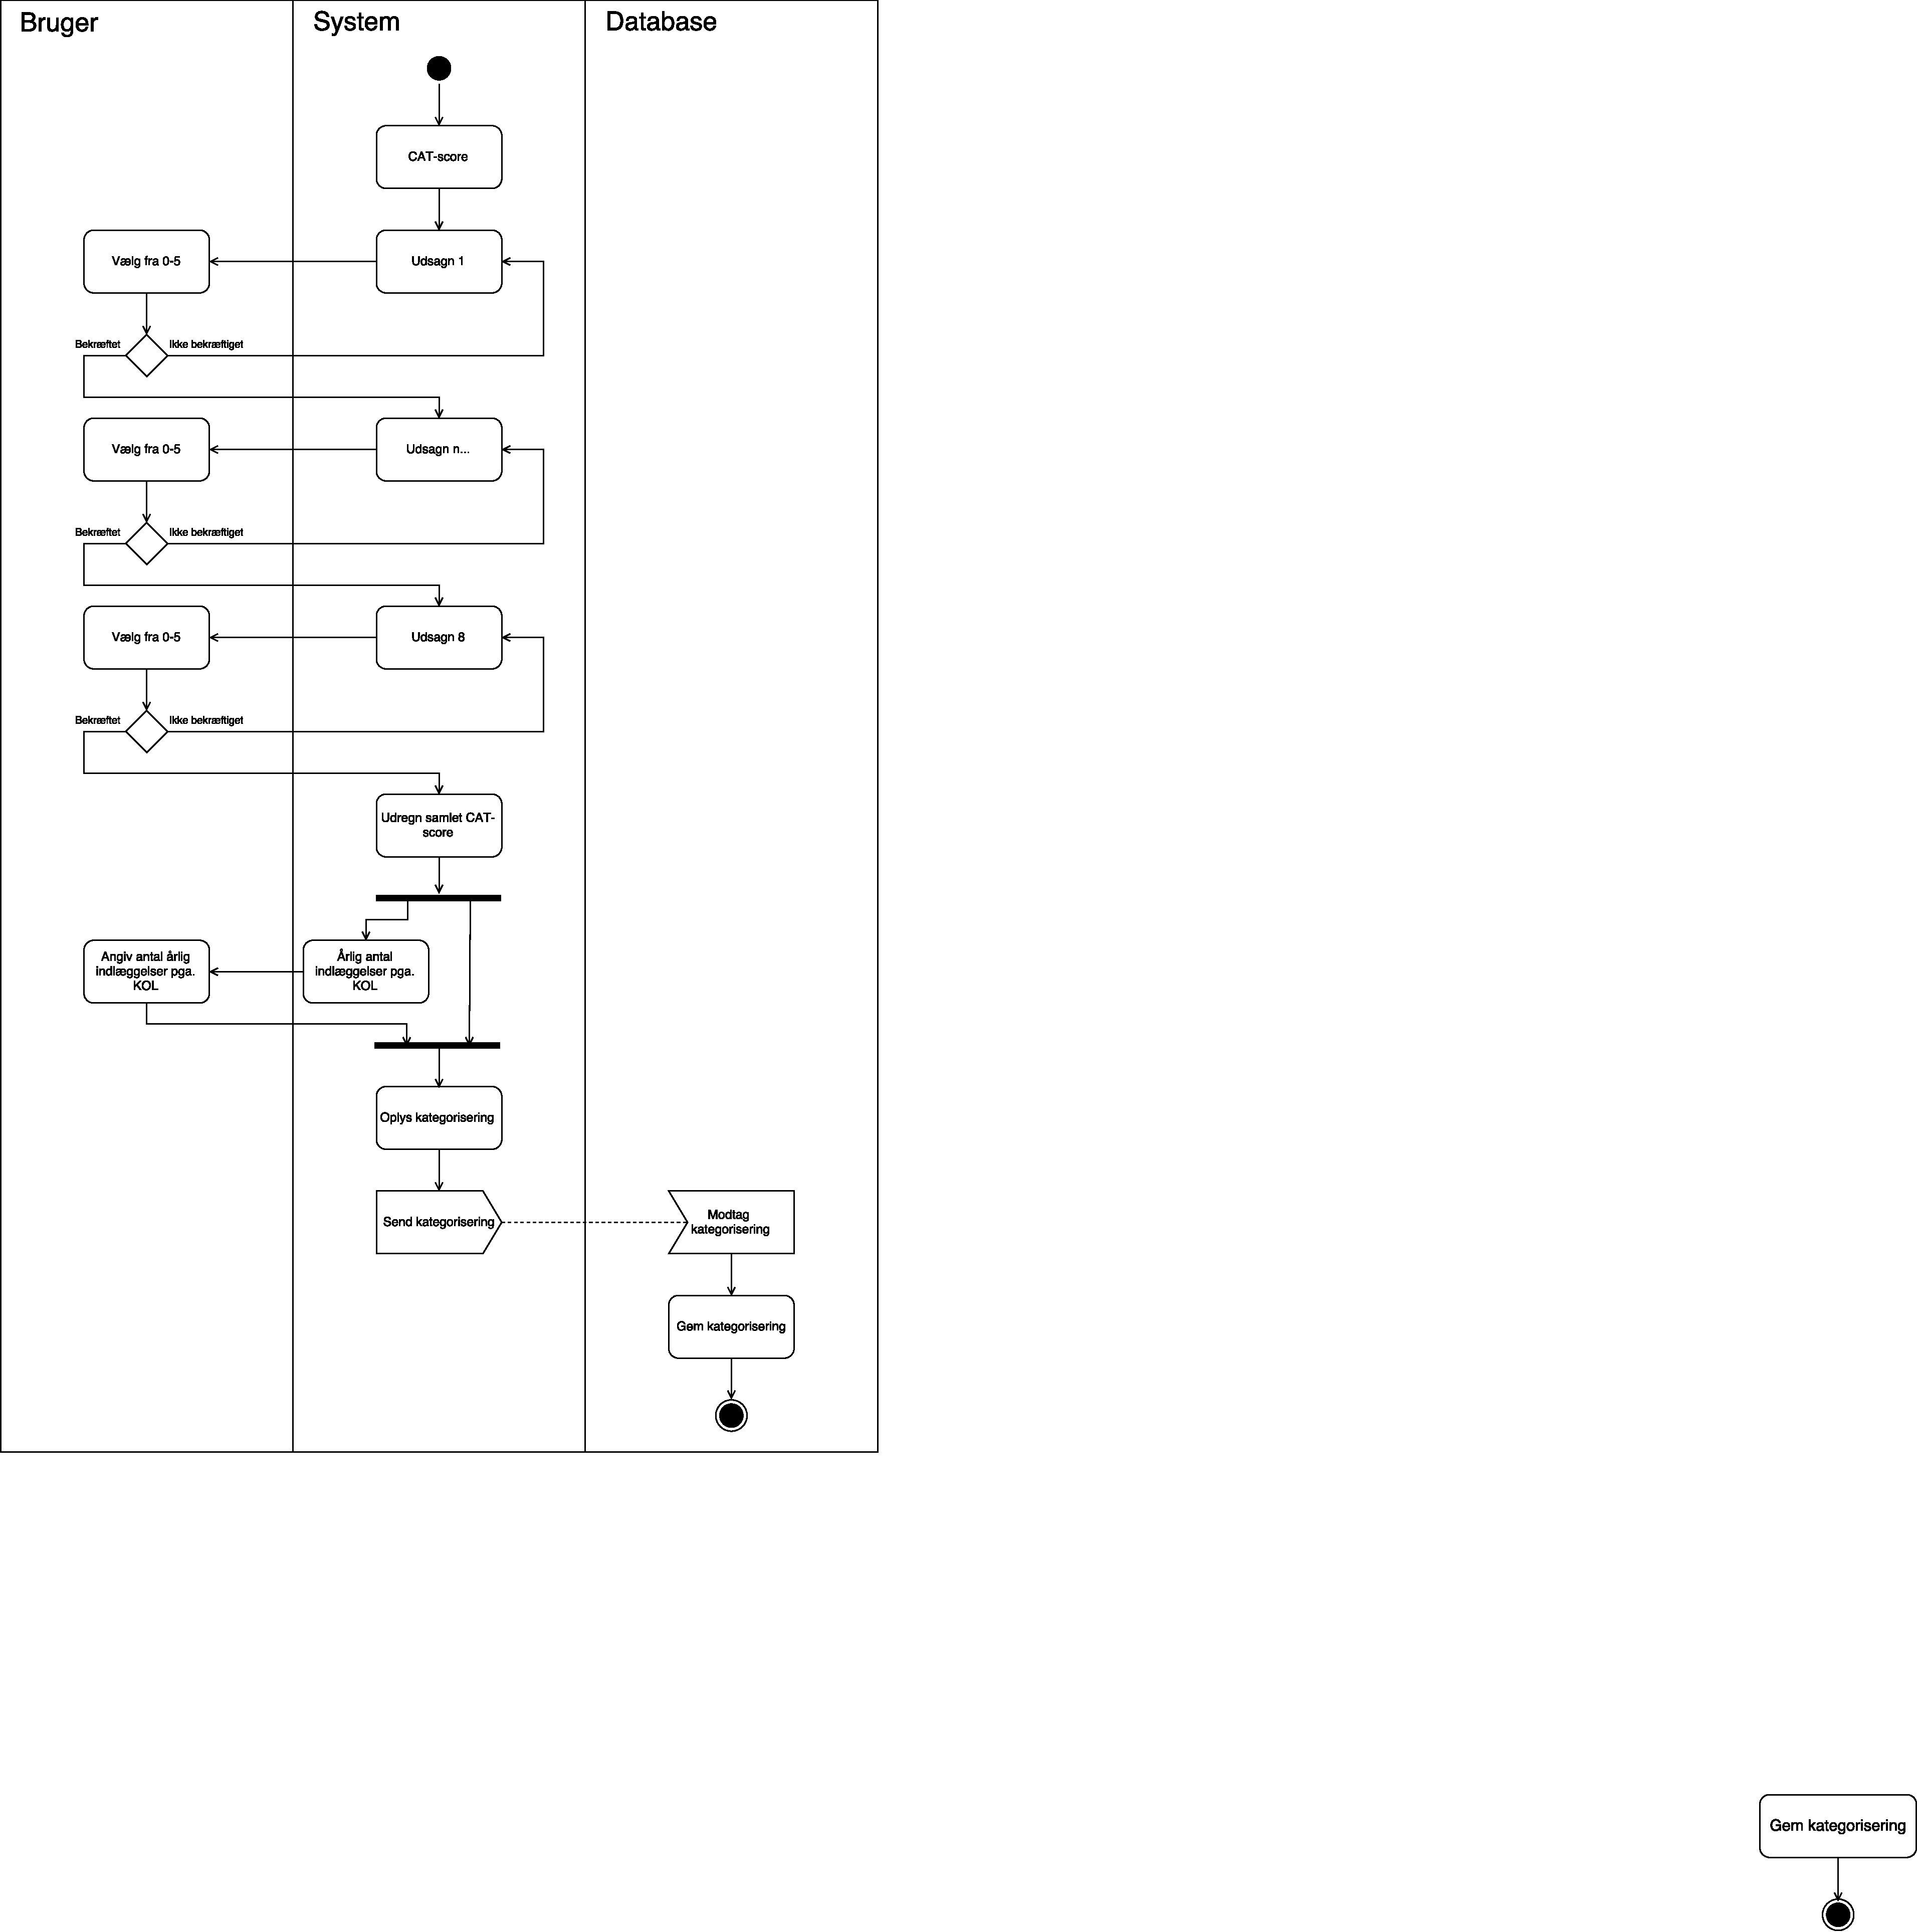
\includegraphics[width=0.65\textwidth]{figures/aktivitetsdiagram/Kategorisering}
\caption{Aktivitetsdiagram for kategorisering af KOL-patienter.}
\label{fig:Kate}
\end{figure}

\noindent
Brugeren stilles otte udsagn, jf. \autoref{fig:CAT}, hvorved de vurderer deres tilstand fra 0 til 5. Tilstanden skal herefter bekræftes af brugeren, hvis det ikke bekræftes stilles det førhenværende udsagn igen. På baggrund af vurderingen fra udsagnene udregnes den samlede CAT-score. Herefter skal brugeren angive antal indlæggelser forårsaget af KOL inden for det seneste år som værende ingen eller én til flere indlæggelser. Ud fra den samlede CAT-score samt de årlige indlæggelser oplyses ABCD-kategoriseringen af patienten. 